\documentclass{article}
\usepackage[a4paper, margin=2cm]{geometry}
\usepackage{parskip}
\setlength{\parskip}{1.5em}

% Math packages
\usepackage{amsthm, commath, bm}

% Physics stuff
\usepackage{physics}

% Graphics
\usepackage{tikz}
\usetikzlibrary{calc, positioning, arrows.meta, decorations.pathmorphing, decorations.text, decorations.pathreplacing, patterns}
\tikzset{
  springcoil/.style={thick, decoration={aspect=0.3, segment length=3mm, amplitude=3mm, coil}, decorate},
}

% Colors
\definecolor{xred}{HTML}{BD4242}
\definecolor{xblue}{HTML}{4268BD}
\definecolor{xgreen}{HTML}{52B256}
\definecolor{xpurple}{HTML}{7F52B2}
\definecolor{xorange}{HTML}{FD9337}
\definecolor{xdotted}{HTML}{999999}
\definecolor{xgray}{HTML}{777777}
\definecolor{xcyan}{HTML}{80F5DC}
\definecolor{xpink}{HTML}{F690EA}
\definecolor{xgrayblue}{HTML}{49B095}
\definecolor{xgraycyan}{HTML}{5AA1B9}

\colorlet{xdarkred}{xred!50!black}
\colorlet{xdarkblue}{xblue!50!black}
\colorlet{xdarkgreen}{xgreen!50!black}
\colorlet{xdarkpurple}{xpurple!50!black}
\colorlet{xdarkorange}{xorange!50!black}

% \usepackage{enumitem}

% Font-related stuff
\usepackage{fontawesome}

% Fancy environments
\usepackage[most]{tcolorbox}
\newenvironment{descitemize}
{\begin{description}[leftmargin=*, before=\let\makelabel\descitemlabel]}
{\end{description}}
\newcommand{\descitemlabel}[1]{\textbullet\ \textbf{#1}:}

\usepackage[most]{tcolorbox}

\tikzset{
	second box/.style={
		anchor=east,
		text=white,
		% rounded corners,
		fill=#1,
		xshift=-4mm,
	},
}
\tikzset{tcbreak/.style = {fill=white, thick, draw=#1, text=#1, font=\bfseries}}
\tcbset{
	common/.style n args={2}{
		colframe={#1},
		colback={#1!5},
		colbacktitle={#1},
		lower separated=false,
		coltitle=white,
		boxrule=1pt,
		fonttitle=\bfseries,
		enhanced,
		breakable,
		top=8pt,
		sharp corners,
		before skip=1em,
		after skip=2em,
		attach boxed title to top left={
			yshift=-0.25cm,
			xshift=0.38cm,
		},
		boxed title style={
			boxrule=0pt,
			colframe=white,
			arc=0pt,
			outer arc=0pt,
		},
		separator sign={~~},
		% -- overlays based on the following TeX SE answer: https://tex.stackexchange.com/a/545324/162087
		overlay unbroken={
			\node[text=white, align=right, fill=#1, xshift=-4mm, minimum height=6mm, anchor=east] at (frame.south east) {#2};
		},
		overlay first={
			\draw[thick, #1, decoration={coil, amplitude=0.5mm}, decorate]
				(frame.south west) -- (frame.south east);
			\path[font=\small\itshape] (frame.south) node [tcbreak={#1}] (cont) {continues in the next page \faHandORight};
		},
		overlay middle={%
			% upper break
			\draw[thick, #1, decoration={coil, amplitude=0.5mm}, decorate]
				(frame.north west) -- (frame.north east);
			\path[font=\small\itshape] (frame.north) node [tcbreak={#1}] (cont) {\faHandORight continues from the previous page};

			% lower break
			\draw[thick, #1, decoration={coil, amplitude=0.5mm}, decorate]
				(frame.south west) -- (frame.south east);
			\path[font=\small\itshape] (frame.south) node [tcbreak={#1}] (cont) {continues in the next page \faHandORight};
		},
		overlay last={
			\node[text=white, align=right, fill=#1, xshift=-4mm, minimum height=6mm, anchor=east] at (frame.south east) {#2};
			\draw[thick, #1, decoration={coil, amplitude=0.5mm}, decorate]
				(frame.north west) -- (frame.north east);
			\path[font=\small\itshape] (frame.north) node [tcbreak={#1}] (cont) {\faHandORight continues from the previous page};
		}
	},
	defstyle/.style={
		common={xpurple}{$\bm{\pi}$},
	},
	theoremstyle/.style={
		common={xgraycyan}{$\multimapdotbothA$},
	},
	lemmastyle/.style={
		common={xgrayblue}{$\multimap$},
	},
	proofstyle/.style={
		common={xgreen}{\textbf{QED}},
	},
	examplestyle/.style={
		common={xblue}{\faStar},
	},
	notestyle/.style={
		common={xred}{\textbf{!}},
	},
	challengestyle/.style={
		common={xgreen}{\textbf{?}},
	},
	quotestyle/.style={
		common={gray}{\textbf{"}},
	},
}

\newtcbtheorem[auto counter, number within=section]{definition}{Definition}{defstyle}{def}
\newtcbtheorem[auto counter, number within=section]{theorem}{Theorem}{theoremstyle}{theorem}
\newtcbtheorem[auto counter, number within=section]{lemma}{Lemma}{lemmastyle}{lemma}
% \newtcbtheorem[auto counter, number within=section]{proof}{Proof}{proofstyle}{proof}
\newtcbtheorem[auto counter, number within=section]{example}{Example}{examplestyle}{example}
\newtcbtheorem[auto counter, number within=section]{note}{Note}{notestyle}{note}
\newtcbtheorem[auto counter, number within=section]{challenge}{Challenge}{challengestyle}{challenge}

% For code samples
\usepackage{listings}

%
\usepackage{booktabs}
\usepackage{hyperref}
% \usepackage{cleveref}

% Text stuff
\usepackage{csquotes}

% Content related-stuff
\title{Course: Physics Simulations\\Lecture Notes}
% NOTE: add mote details!
\author{Peleg Bar Sapir}

%%%% MAIN DOC %%%%

\begin{document}
\maketitle

% For tests
\ifdefined\testcode
  \section{Tests}
  This is a test. And this is a reference to some code: \autoref{lst:code1}.
  \begin{lstlisting}[
	% there are many more options of styling, see the official documentation, these are just the defaults I like
	frame=single, % make single-line frame around the verbatim
	framesep=2mm, % put some more spacing between the frame and text
	aboveskip=5mm, % put some more space above the box
	basicstyle={\linespread{0.9}\small\ttfamily}, % use typewriter (monospace) font
	caption={I am some code.}, % set the caption text
	captionpos=b, % put the caption at the bottom (b) or top (t) or both (bt)
	label={lst:code1}, % label to be referenced via \ref{}
	numbers=left, % line numbers on the left
	numberstyle={\scriptsize\ttfamily\color{black!60}}, % the style for line numbers
	escapeinside={<@}{@>} % between those sequences are command evaluated
]
<@\textcolor[HTML]{3010CF}{\textit{\textbf{\texttt{import}}}}@><@\textcolor[HTML]{000000}{\texttt{\ }}@><@\textcolor[HTML]{000000}{\texttt{numpy}}@><@\textcolor[HTML]{000000}{\texttt{\ }}@><@\textcolor[HTML]{3010CF}{\textit{\textbf{\texttt{as}}}}@><@\textcolor[HTML]{000000}{\texttt{\ }}@><@\textcolor[HTML]{000000}{\texttt{np}}@>
<@\textcolor[HTML]{3010CF}{\textit{\textbf{\texttt{import}}}}@><@\textcolor[HTML]{000000}{\texttt{\ }}@><@\textcolor[HTML]{000000}{\texttt{numpy}}@><@\textcolor[HTML]{000000}{\texttt{.}}@><@\textcolor[HTML]{000000}{\texttt{typing}}@><@\textcolor[HTML]{000000}{\texttt{\ }}@><@\textcolor[HTML]{3010CF}{\textit{\textbf{\texttt{as}}}}@><@\textcolor[HTML]{000000}{\texttt{\ }}@><@\textcolor[HTML]{000000}{\texttt{npt}}@>


<@\textcolor[HTML]{777777}{\textit{\texttt{\#\ Axes}}}@>
<@\textcolor[HTML]{EA5110}{\texttt{X\_}}@><@\textcolor[HTML]{000000}{\texttt{,\ }}@><@\textcolor[HTML]{EA5110}{\texttt{Y\_}}@><@\textcolor[HTML]{000000}{\texttt{,\ }}@><@\textcolor[HTML]{EA5110}{\texttt{Z\_}}@><@\textcolor[HTML]{000000}{\texttt{\ }}@><@\textcolor[HTML]{1041FF}{\texttt{=}}@><@\textcolor[HTML]{000000}{\texttt{\ }}@><@\textcolor[HTML]{000000}{\texttt{np}}@><@\textcolor[HTML]{000000}{\texttt{.}}@><@\textcolor[HTML]{2387FF}{\texttt{ones}}@><@\textcolor[HTML]{000000}{\texttt{(}}@><@\textcolor[HTML]{DE6F10}{\texttt{3}}@><@\textcolor[HTML]{000000}{\texttt{)}}@>
<@\textcolor[HTML]{000000}{\texttt{}}@>
<@\textcolor[HTML]{777777}{\textit{\texttt{\#\ NumPy\ types}}}@>
<@\textcolor[HTML]{724BFF}{\textit{\texttt{NDArrayFloat}}}@><@\textcolor[HTML]{000000}{\texttt{\ }}@><@\textcolor[HTML]{1041FF}{\texttt{=}}@><@\textcolor[HTML]{000000}{\texttt{\ }}@><@\textcolor[HTML]{000000}{\texttt{npt}}@><@\textcolor[HTML]{000000}{\texttt{.}}@><@\textcolor[HTML]{2387FF}{\texttt{NDArray}}@><@\textcolor[HTML]{000000}{\texttt{[}}@><@\textcolor[HTML]{000000}{\texttt{np}}@><@\textcolor[HTML]{000000}{\texttt{.}}@><@\textcolor[HTML]{2387FF}{\texttt{float\_}}@><@\textcolor[HTML]{000000}{\texttt{]}}@>
<@\textcolor[HTML]{000000}{\texttt{}}@>

<@\textcolor[HTML]{777777}{\textit{\texttt{\#\ Functions}}}@>
<@\textcolor[HTML]{3010CF}{\textit{\textbf{\texttt{def}}}}@><@\textcolor[HTML]{000000}{\texttt{\ }}@><@\textcolor[HTML]{255CFF}{\texttt{normalize}}@><@\textcolor[HTML]{000000}{\texttt{(}}@><@\textcolor[HTML]{000000}{\texttt{vec}}@><@\textcolor[HTML]{000000}{\texttt{:\ }}@><@\textcolor[HTML]{1F8F42}{\texttt{NDArrayFloat}}@><@\textcolor[HTML]{000000}{\texttt{)\ }}@><@\textcolor[HTML]{1041FF}{\texttt{->}}@><@\textcolor[HTML]{000000}{\texttt{\ }}@><@\textcolor[HTML]{1F8F42}{\texttt{NDArrayFloat}}@><@\textcolor[HTML]{000000}{\texttt{:}}@>
<@\textcolor[HTML]{000000}{\texttt{}}@><@\textcolor[HTML]{000000}{\texttt{\ \ \ \ }}@><@\textcolor[HTML]{EA5110}{\texttt{L}}@><@\textcolor[HTML]{000000}{\texttt{:\ }}@><@\textcolor[HTML]{1F8F42}{\texttt{float}}@><@\textcolor[HTML]{000000}{\texttt{\ }}@><@\textcolor[HTML]{1041FF}{\texttt{=}}@><@\textcolor[HTML]{000000}{\texttt{\ }}@><@\textcolor[HTML]{000000}{\texttt{np}}@><@\textcolor[HTML]{000000}{\texttt{.}}@><@\textcolor[HTML]{2387FF}{\texttt{linalg}}@><@\textcolor[HTML]{000000}{\texttt{.}}@><@\textcolor[HTML]{2387FF}{\texttt{norm}}@><@\textcolor[HTML]{000000}{\texttt{(}}@><@\textcolor[HTML]{000000}{\texttt{vec}}@><@\textcolor[HTML]{000000}{\texttt{)}}@>
<@\textcolor[HTML]{000000}{\texttt{}}@><@\textcolor[HTML]{000000}{\texttt{\ \ \ \ }}@><@\textcolor[HTML]{3010CF}{\textit{\textbf{\texttt{assert}}}}@><@\textcolor[HTML]{000000}{\texttt{\ }}@><@\textcolor[HTML]{EA5110}{\texttt{L}}@><@\textcolor[HTML]{000000}{\texttt{\ }}@><@\textcolor[HTML]{1041FF}{\texttt{!=}}@><@\textcolor[HTML]{000000}{\texttt{\ }}@><@\textcolor[HTML]{DE6F10}{\texttt{0.}}@><@\textcolor[HTML]{000000}{\texttt{,\ }}@><@\textcolor[HTML]{418310}{\texttt{"Can't\ normalize\ the\ zero\ vector."}}@>
<@\textcolor[HTML]{000000}{\texttt{\ \ \ \ }}@><@\textcolor[HTML]{3010CF}{\textit{\textbf{\texttt{return}}}}@><@\textcolor[HTML]{000000}{\texttt{\ }}@><@\textcolor[HTML]{000000}{\texttt{vec}}@><@\textcolor[HTML]{000000}{\texttt{\ }}@><@\textcolor[HTML]{1041FF}{\texttt{/}}@><@\textcolor[HTML]{000000}{\texttt{\ }}@><@\textcolor[HTML]{EA5110}{\texttt{L}}@>


<@\textcolor[HTML]{3010CF}{\textit{\textbf{\texttt{def}}}}@><@\textcolor[HTML]{000000}{\texttt{\ }}@><@\textcolor[HTML]{255CFF}{\texttt{scale}}@><@\textcolor[HTML]{000000}{\texttt{(}}@><@\textcolor[HTML]{000000}{\texttt{vec}}@><@\textcolor[HTML]{000000}{\texttt{:\ }}@><@\textcolor[HTML]{1F8F42}{\texttt{NDArrayFloat}}@><@\textcolor[HTML]{000000}{\texttt{,\ }}@><@\textcolor[HTML]{000000}{\texttt{a}}@><@\textcolor[HTML]{000000}{\texttt{:\ }}@><@\textcolor[HTML]{1F8F42}{\texttt{float}}@><@\textcolor[HTML]{000000}{\texttt{)\ }}@><@\textcolor[HTML]{1041FF}{\texttt{->}}@><@\textcolor[HTML]{000000}{\texttt{\ }}@><@\textcolor[HTML]{1F8F42}{\texttt{NDArrayFloat}}@><@\textcolor[HTML]{000000}{\texttt{:}}@>
<@\textcolor[HTML]{000000}{\texttt{}}@><@\textcolor[HTML]{000000}{\texttt{\ \ \ \ }}@><@\textcolor[HTML]{3010CF}{\textit{\textbf{\texttt{return}}}}@><@\textcolor[HTML]{000000}{\texttt{\ }}@><@\textcolor[HTML]{255CFF}{\texttt{normalize}}@><@\textcolor[HTML]{000000}{\texttt{(}}@><@\textcolor[HTML]{000000}{\texttt{vec}}@><@\textcolor[HTML]{000000}{\texttt{)\ }}@><@\textcolor[HTML]{1041FF}{\texttt{*}}@><@\textcolor[HTML]{000000}{\texttt{\ }}@><@\textcolor[HTML]{000000}{\texttt{a}}@>

\end{lstlisting}


  And this is a TikZ drawing: \autoref{fig:tikztest}.

  \begin{figure}
      \begin{center}
      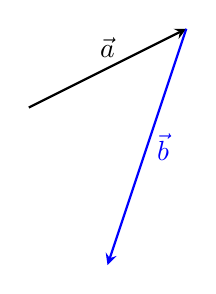
\begin{tikzpicture}
        \draw[-stealth, thick] (0,0) -- (2,1) node[midway, above] {$\vec{a}$};
        \draw[-stealth, thick, blue] (2,1) -- ++(-1,-3) node[midway, right] {$\vec{b}$};
      \end{tikzpicture}
      \end{center}
    \caption{A figure.}\label{fig:tikztest}
  \end{figure}
  
\else
\fi

% Content
\section{Introduction}
\subsection{Why are Simulations Used?}
\subsection{Python}
\subsection{A Bit About Git}
\subsection{Some Mathematical Background}

\section{Simulating Simple Mechanics}
\subsection{Forward Euler Method}
\subsection{Backward Euler Method}
\subsection{Verlet Integration}
\subsection{Runge-Kutta Method}

\section{Thermodynamics}

\section{Waves}

\section{Molecular Dynamics}


\end{document}
